\documentclass[letterpaper,10pt]{article}
\usepackage[top=2cm, bottom=1.5cm, left=1cm, right=1cm]{geometry}
\usepackage{amsmath, amssymb, amsthm,graphicx}
\usepackage{fancyhdr}
\pagestyle{fancy}

\lhead{March 15, 2019}
\chead{Meeting 4}
\rhead{Justin Hood}

\newcommand{\Z}{\mathbb{Z}}
\newcommand{\Q}{\mathbb{Q}}
\newcommand{\R}{\mathbb{R}}
\newcommand{\C}{\mathbb{C}}
\newcommand{\NORM}{\Big|\Big|}
\newtheorem{lem}{Lemma}

\begin{document}
\begin{enumerate}
\item Webwork Completed.
\item We consider the linear system,
\begin{align*}
x_1-x_2+\alpha x_3 &= -2\\
-x_1+2x_2-\alpha x_3 &= 3\\
\alpha x_1+x_2+x_3 &= 2
\end{align*}
Translating this into matrix form,
\[\begin{bmatrix}
1 & -1 & \alpha\\
-1 & 2 & -\alpha\\
\alpha & 1 & 1
\end{bmatrix}\begin{bmatrix}
x_1\\x_2\\x_3
\end{bmatrix}=\begin{bmatrix}
-2\\3\\2
\end{bmatrix} \]
We consider reducing the augmented matrix as,
\begin{align*}
\left[\begin{array}{ccc|c}
1 & -1 & \alpha & -2\\
-1 & 2 & -\alpha & 3\\
\alpha & 1 & 1 & 2
\end{array}\right] &= \left[\begin{array}{ccc|c}
1 & -1 & \alpha & -2\\
0 & 1 & 0 & 1\\
\alpha & 1 & 1 & 2
\end{array}\right] && R_2+R_1\to R_2\\
&=  \left[\begin{array}{ccc|c}
1 & 0 & \alpha & -1\\
0 & 1 & 0 & 1\\
\alpha & 0 & 1 & 1
\end{array}\right] && R_1+R_2\to R_1,\ R_3-R_2\to R_3
\end{align*}
From this form, we see that the critical values of $\alpha$ are $\pm 1$. Now,
\begin{enumerate}
\item First, we consider $\alpha=1$. Our augmented matrix is then,
\[\left[\begin{array}{ccc|c}
1 & 0 & 1 & -1\\
0 & 1 & 0 & 1\\
1 & 0 & 1 & 1
\end{array}\right]\]
Which is clearly an impossibility. So, we see that there are no solutions of the system when $\alpha =1$.
\item Next, consider $\alpha=-1$. Our augmented matrix is then,
\[\left[\begin{array}{ccc|c}
1 & 0 & -1 & -1\\
0 & 1 & 0 & 1\\
-1 & 0 & 1 & 1
\end{array}\right]=\left[\begin{array}{ccc|c}
1 & 0 & -1 & -1\\
0 & 1 & 0 & 1\\
0 & 0 & 0 & 0
\end{array}\right]\]
Because we have fewer pivots than variables, we see that we have an infinite space of solutions, depending on our choice of either $x_1$ or $x_3$.
\item Finally, we consider the case where $\alpha \neq \pm 1$. Here, we shall reduce the augmented matrix to reduced row echelon form to find our ``Solution Vector". Here, the result is,
\[\left[\begin{array}{ccc|c}
1 & 0 & \alpha & -1\\
0 & 1 & 0 & 1\\
\alpha & 0 & 1 & 1
\end{array}\right]=\left[\begin{array}{ccc|c}
1 & 0 & 0 & -1-\frac{\alpha(1+\alpha)}{1-\alpha^2}\\
0 & 1 & 0 & 1\\
0 & 0 & 1 & \frac{1+\alpha}{1-\alpha^2}
\end{array}\right] \]
So, for a given $\alpha$, the solution is,
\[\vec{X}=\begin{bmatrix}
-1-\frac{\alpha(1+\alpha)}{1-\alpha^2}\\
1\\
\frac{1+\alpha}{1-\alpha^2}
\end{bmatrix} \]
\end{enumerate}
\item See Jupyter Notebook
\item We consider an arbitrary matrix $B$ with dimension $4\times 4$. We note that multiplications on the left of the original matrix affect the rows of the resultant matrix, and multiplications to the right affect the columns. So, we consider the operations from the text which are noted with braces below,
\begin{enumerate}
\item Double Column 1,
\[B\underbrace{\begin{bmatrix}
2 & 0 & 0 & 0\\
0 & 1 & 0 & 0\\
0 & 0 & 1 & 0\\
0 & 0 & 0 & 1
\end{bmatrix}} \]
\item Halve Row 3,
\[\underbrace{\begin{bmatrix}
1 & 0 & 0 & 0\\
0 & 1 & 0 & 0\\
0 & 0 & \frac{1}{2} & 0\\
0 & 0 & 0 & 1
\end{bmatrix}}B\begin{bmatrix}
2 & 0 & 0 & 0\\
0 & 1 & 0 & 0\\
0 & 0 & 1 & 0\\
0 & 0 & 0 & 1
\end{bmatrix} \]
\item Add Row 3 to Row 1,
\[\underbrace{\begin{bmatrix}
1 & 0 & 1 & 0\\
0 & 1 & 0 & 0\\
0 & 0 & 1 & 0\\
0 & 0 & 0 & 1
\end{bmatrix}} \begin{bmatrix}
1 & 0 & 0 & 0\\
0 & 1 & 0 & 0\\
0 & 0 & \frac{1}{2} & 0\\
0 & 0 & 0 & 1
\end{bmatrix}B\begin{bmatrix}
2 & 0 & 0 & 0\\
0 & 1 & 0 & 0\\
0 & 0 & 1 & 0\\
0 & 0 & 0 & 1
\end{bmatrix} \]
\item Interchange Column 4 and Column 1,
\[\begin{bmatrix}
1 & 0 & 1 & 0\\
0 & 1 & 0 & 0\\
0 & 0 & 1 & 0\\
0 & 0 & 0 & 1
\end{bmatrix} \begin{bmatrix}
1 & 0 & 0 & 0\\
0 & 1 & 0 & 0\\
0 & 0 & \frac{1}{2} & 0\\
0 & 0 & 0 & 1
\end{bmatrix}B\begin{bmatrix}
2 & 0 & 0 & 0\\
0 & 1 & 0 & 0\\
0 & 0 & 1 & 0\\
0 & 0 & 0 & 1
\end{bmatrix} \underbrace{\begin{bmatrix}
0 & 0 & 0 & 1\\
0 & 1 & 0 & 0\\
0 & 0 & 1 & 0\\
1 & 0 & 0 & 0
\end{bmatrix}} \]
\item Subtract Row 2 from the other rows,
\[\underbrace{\begin{bmatrix}
1 & -1 & 0 & 0\\
0 & 1 & 0 & 0\\
0 & -1 & 1 & 0\\
0 & -1 & 0 & 1
\end{bmatrix}} \begin{bmatrix}
1 & 0 & 1 & 0\\
0 & 1 & 0 & 0\\
0 & 0 & 1 & 0\\
0 & 0 & 0 & 1
\end{bmatrix} \begin{bmatrix}
1 & 0 & 0 & 0\\
0 & 1 & 0 & 0\\
0 & 0 & \frac{1}{2} & 0\\
0 & 0 & 0 & 1
\end{bmatrix}B\begin{bmatrix}
2 & 0 & 0 & 0\\
0 & 1 & 0 & 0\\
0 & 0 & 1 & 0\\
0 & 0 & 0 & 1
\end{bmatrix} \begin{bmatrix}
0 & 0 & 0 & 1\\
0 & 1 & 0 & 0\\
0 & 0 & 1 & 0\\
1 & 0 & 0 & 0
\end{bmatrix} \]
\item Replace Column 4 with Column 3,
\[\begin{bmatrix}
1 & -1 & 0 & 0\\
0 & 1 & 0 & 0\\
0 & -1 & 1 & 0\\
0 & -1 & 0 & 1
\end{bmatrix} \begin{bmatrix}
1 & 0 & 1 & 0\\
0 & 1 & 0 & 0\\
0 & 0 & 1 & 0\\
0 & 0 & 0 & 1
\end{bmatrix} \begin{bmatrix}
1 & 0 & 0 & 0\\
0 & 1 & 0 & 0\\
0 & 0 & \frac{1}{2} & 0\\
0 & 0 & 0 & 1
\end{bmatrix}B\begin{bmatrix}
2 & 0 & 0 & 0\\
0 & 1 & 0 & 0\\
0 & 0 & 1 & 0\\
0 & 0 & 0 & 1
\end{bmatrix} \begin{bmatrix}
0 & 0 & 0 & 1\\
0 & 1 & 0 & 0\\
0 & 0 & 1 & 0\\
1 & 0 & 0 & 0
\end{bmatrix} \underbrace{\begin{bmatrix}
1 & 0 & 0 & 0\\
0 & 1 & 0 & 0\\
0 & 0 & 1 & 1\\
0 & 0 & 0 & 0
\end{bmatrix}}\]
\item Delete Column 1,
\[\begin{bmatrix}
1 & -1 & 0 & 0\\
0 & 1 & 0 & 0\\
0 & -1 & 1 & 0\\
0 & -1 & 0 & 1
\end{bmatrix} \begin{bmatrix}
1 & 0 & 1 & 0\\
0 & 1 & 0 & 0\\
0 & 0 & 1 & 0\\
0 & 0 & 0 & 1
\end{bmatrix} \begin{bmatrix}
1 & 0 & 0 & 0\\
0 & 1 & 0 & 0\\
0 & 0 & \frac{1}{2} & 0\\
0 & 0 & 0 & 1
\end{bmatrix}B\begin{bmatrix}
2 & 0 & 0 & 0\\
0 & 1 & 0 & 0\\
0 & 0 & 1 & 0\\
0 & 0 & 0 & 1
\end{bmatrix} \begin{bmatrix}
0 & 0 & 0 & 1\\
0 & 1 & 0 & 0\\
0 & 0 & 1 & 0\\
1 & 0 & 0 & 0
\end{bmatrix} \begin{bmatrix}
1 & 0 & 0 & 0\\
0 & 1 & 0 & 0\\
0 & 0 & 1 & 1\\
0 & 0 & 0 & 0
\end{bmatrix}\underbrace{\begin{bmatrix}
0 & 0 & 0\\
1 & 0 & 0\\
0 & 1 & 0\\
0 & 0 & 1
\end{bmatrix}}\]
\end{enumerate}
Now, we compute the $A$ matrix as,
\[A=\begin{bmatrix}
1 & -1 & 0 & 0\\
0 & 1 & 0 & 0\\
0 & -1 & 1 & 0\\
0 & -1 & 0 & 1
\end{bmatrix} \begin{bmatrix}
1 & 0 & 1 & 0\\
0 & 1 & 0 & 0\\
0 & 0 & 1 & 0\\
0 & 0 & 0 & 1
\end{bmatrix} \begin{bmatrix}
1 & 0 & 0 & 0\\
0 & 1 & 0 & 0\\
0 & 0 & \frac{1}{2} & 0\\
0 & 0 & 0 & 1
\end{bmatrix}=\begin{bmatrix}
1 & -1 & \frac{1}{2} & 0\\
0 & 1 & 0 & 0\\
0 & -1 & \frac{1}{2} & 0\\
0 & -1 & 0 & 1
\end{bmatrix} \]
And matrix $C$ as,
\[C=\begin{bmatrix}
2 & 0 & 0 & 0\\
0 & 1 & 0 & 0\\
0 & 0 & 1 & 0\\
0 & 0 & 0 & 1
\end{bmatrix} \begin{bmatrix}
0 & 0 & 0 & 1\\
0 & 1 & 0 & 0\\
0 & 0 & 1 & 0\\
1 & 0 & 0 & 0
\end{bmatrix} \begin{bmatrix}
1 & 0 & 0 & 0\\
0 & 1 & 0 & 0\\
0 & 0 & 1 & 1\\
0 & 0 & 0 & 0
\end{bmatrix}\begin{bmatrix}
0 & 0 & 0\\
1 & 0 & 0\\
0 & 1 & 0\\
0 & 0 & 1
\end{bmatrix}=\begin{bmatrix}
0 & 0 & 0\\
1 & 0 & 0\\
0 & 1 & 1\\
0 & 0 & 0
\end{bmatrix} \]
Thus,
\[ABC=\begin{bmatrix}
1 & -1 & \frac{1}{2} & 0\\
0 & 1 & 0 & 0\\
0 & -1 & \frac{1}{2} & 0\\
0 & -1 & 0 & 1
\end{bmatrix}B\begin{bmatrix}
0 & 0 & 0\\
1 & 0 & 0\\
0 & 1 & 1\\
0 & 0 & 0
\end{bmatrix} \]
\item Let us consider a matrix $R$ which is non-singular and upper triangular. We write $R$ as,
\[R=\begin{bmatrix}
r_{11} & r_{12} & \cdots & r_{1m}\\
0 & r_{22} & \cdots & r_{2m}\\
\vdots & \vdots & \ddots & \vdots\\
0 & 0 & \cdots & r_{mm}
\end{bmatrix} \]
Now, noting that $R$ is defined to be non-singular, we note that $det(R)\neq 0$. Given its triangular nature, we know that $det(R)=r_{11}r_{22}\ldots r_{mm}$, thus, each of these diagonal entries must be non-zero as well. Now, we note as from the previous problem that we can perform row wise operations on $R$ by premultiplying matrices that encode the operations. As such, we consider how that might be done. First, we scale the diagonal elements,
\[\begin{bmatrix}
1 & \frac{r_{12}}{r_{11}} & \cdots & \frac{r_{1m}}{r_{11}}\\
0 & 1 & \cdots & \frac{r_{2m}}{r_{22}}\\
\vdots & \vdots & \ddots & \vdots\\
0 & 0 & \cdots & 1
\end{bmatrix}=\begin{bmatrix}
\frac{1}{r_{11}} & 0 & \cdots & 0\\
0 & \frac{1}{r_{22}} & \cdots & 0\\
\vdots & \vdots & \ddots & \vdots\\
0 & 0 & \cdots & \frac{1}{r_{mm}}
\end{bmatrix}\begin{bmatrix}
r_{11} & r_{12} & \cdots & r_{1m}\\
0 & r_{22} & \cdots & r_{2m}\\
\vdots & \vdots & \ddots & \vdots\\
0 & 0 & \cdots & r_{mm}
\end{bmatrix} \]
From this result, we see that the matrix can easlily be reduced to the identity by continuing to reduce each of the columns individually. Starting with the $m$th column and working backward to the first, we subtract the scaled factor for the corresponding column. For the $m$th column, we compute,
\[\begin{bmatrix}
1 & \frac{r_{12}}{r_{11}} & \cdots & 0\\
0 & 1 & \cdots & 0\\
\vdots & \vdots & \ddots & \vdots\\
0 & 0 & \cdots & 1
\end{bmatrix}=\begin{bmatrix}
1 & 0 & \cdots & -\frac{r_{1m}}{r_{11}}\\
0 & 1 & \cdots & -\frac{r_{2m}}{r_{22}}\\
\vdots & \vdots & \ddots & \vdots\\
0 & 0 & \cdots & 1
\end{bmatrix} \begin{bmatrix}
\frac{1}{r_{11}} & 0 & \cdots & 0\\
0 & \frac{1}{r_{22}} & \cdots & 0\\
\vdots & \vdots & \ddots & \vdots\\
0 & 0 & \cdots & \frac{1}{r_{mm}}
\end{bmatrix}\begin{bmatrix}
r_{11} & r_{12} & \cdots & r_{1m}\\
0 & r_{22} & \cdots & r_{2m}\\
\vdots & \vdots & \ddots & \vdots\\
0 & 0 & \cdots & r_{mm}
\end{bmatrix} \]
We see that this scaling matrix is also upper triangular. So,
\[\begin{bmatrix}
1 & \frac{r_{12}}{r_{11}} & \cdots & 0\\
0 & 1 & \cdots & 0\\
\vdots & \vdots & \ddots & \vdots\\
0 & 0 & \cdots & 1
\end{bmatrix}=\underbrace{\begin{bmatrix}
1 & 0 & \cdots & -\frac{r_{1m}}{r_{11}}\\
0 & 1 & \cdots & -\frac{r_{2m}}{r_{22}}\\
\vdots & \vdots & \ddots & \vdots\\
0 & 0 & \cdots & 1
\end{bmatrix} \begin{bmatrix}
\frac{1}{r_{11}} & 0 & \cdots & 0\\
0 & \frac{1}{r_{22}} & \cdots & 0\\
\vdots & \vdots & \ddots & \vdots\\
0 & 0 & \cdots & \frac{1}{r_{mm}}
\end{bmatrix}}_{\text{Upper-Triangular}}\begin{bmatrix}
r_{11} & r_{12} & \cdots & r_{1m}\\
0 & r_{22} & \cdots & r_{2m}\\
\vdots & \vdots & \ddots & \vdots\\
0 & 0 & \cdots & r_{mm}
\end{bmatrix} \]
Repeating this scaling process for the $m-1$th column and on, we see that $R^{-1}$ is the product of upper triangular matrices, and is thus upper triangular as well. 
\item Let $A$ be triangular and unitary. Without loss of generality, let us assume that $A$ is upper triangular. From example 1.3, we know that $A^{-1}$ is also upper triangular. For a unitary matrix, we know that $A^T=A^{-1}$, So, consider the shape of matrix $A$,
\[A=\begin{bmatrix}
a_{11} & a_{12} & \cdots & a_{1m}\\
0 & a_{22} & \cdots & a_{2m}\\
\vdots & \vdots & \ddots & \vdots\\
0 & 0 & \cdots & a_{mm}
\end{bmatrix}\]
Now, consider,
\[A^T=\begin{bmatrix}
a_{11} & 0 & \cdots & 0\\
a_{12} & a_{22} & \cdots & 0\\
\vdots & \vdots & \ddots & \vdots\\
a_{1m} & a_{2m} & \cdots & a_{mm}
\end{bmatrix}=A^{-1} \]
Now, we note that $A^{-1}$ has been shown to be upper triangular. So,
\[A^{-1}=\begin{bmatrix}
a_{11} & 0 & \cdots & 0\\
0 & a_{22} & \cdots & 0\\
\vdots & \vdots & \ddots & \vdots\\
0 & 0 & \cdots & a_{mm}
\end{bmatrix} \]
Thus, we see that $A^{-1}$ must be diagonal. Now, $A^{-1}=A^T$, thus, we conclude that $A$ is also diagonal.
\item Consider the Pythagorean theorem for orthogonal vectors $\{x_i\}$,
\[\NORM\sum_{i=1}^nx_i\NORM^2=\sum_{i=1}^n||x_i||^2\]
\begin{enumerate}
\item Consider the case $n=2$. Then,
\begin{align*}
\NORM\sum_{i=1}^2x_i\NORM^2 &= ||x_1+x_2||^2\\
&=\sum_{i=1}^m(x_{1i}+x_{2i})^2\\
&=\sum_{i=1}^m\left[x_{1i}^2+x_{2i}^2+2x_{1i}x_{2i}\right] && \text{By Orthogonality}\\
&=||x_1||^2+||x_2||^2
\end{align*}
\item Now, we assume, $\NORM \sum_{i=2}^kx_i\NORM^2=\sum_{i=1}^k||x_i||^2$ for $1\leq k \leq n$. Then, consider the $n+1$ case,
\begin{align*}
\NORM\sum_{i=1}^{n+1}x_i\NORM^2 &= \NORM\sum_{i=1}^{n}x_i\NORM^2+||x_{n+1}||^2+\NORM\sum_{i=1}^nx_{i}x_{n+1}\NORM && \text{By orthogonality}\\
&=\sum_{i=1}^n||x_i||^2+||x_{n+1}||^2 && \text{By assumption}\\
&=\sum_{i=1}^{n+1}||x_i||^2
\end{align*}
As desired. Thus, we see that the results hold for an arbitrary $n$.
\end{enumerate}
\item Consider a hermitian matrix $A\in \C^{m\times m}$, and let $x\in \C^m$ be a non-zero eigenvector of $A$, such that, $Ax=\lambda x$ for $\lambda\in \C$. 
\begin{enumerate}
\item Consider,
\[\lambda||x||^2=\lambda x^*x=x^*\lambda x=x^*(Ax)=(x^*A^*)x=(Ax)^*x=(\lambda x)^*x=x^*\lambda^*x=\lambda^*x^*x=\lambda^*||x||^2\]
Here, we see that $\lambda=\lambda^*4$. For a constant value, this may only be true if $IM(\lambda)=0$, i.e. $\lambda\in \R$. So, we see that the eigenvalues are real for this case.
\item Now, let $x$ and $y$ be eigenvectors with eigenvalues, $\lambda$ and $\mu$ respectively, with $\lambda \neq \mu$. So, we have $Ax=\lambda x$ and $Ay=\mu y$. Consider, as before,
\[\lambda y^*x=y^*(\lambda x)=y^*(Ax)=(y^*A)x=(Ay)^*x=(\mu y)^*x=\mu y^*x\]
So, we have,
\[\lambda y^*x=\mu y^*x\]
Since, $\lambda \neq \mu$, we see that $y^*x=0$. So, we see that $x$ and $y$ are orthogonal. 
\end{enumerate}
\item Let $x$ be an $m$-vector and $A$ an $m\times n$ matrix.
\begin{enumerate}
\item Consider $||x||_{\infty}\leq ||x||_2$. Without loss of generality, let $|x_{1}|=\max_{1\leq i\leq m}|x_i|=||x||_{\infty}$. Now, 
\[||x||_2=\sqrt{\sum_{i=1}^m|x_i|^2}=\sqrt{|x_1|^2+|x_2|^2+\ldots+|x_m|^2}\geq |x_i|\]
Thus, we see that $||x||_{\infty}\leq ||x||_2$. For equality, we consider,
\[x=\begin{bmatrix}
1\\0\\0\\\vdots\\ 0
\end{bmatrix}\]
Then,
\[||x||_{\infty}=|1|=\sqrt{|1|^2}=||x||_2\]
\item Consider now, $||x||_2\leq \sqrt{m}||x||_{\infty}$. Again, without loss of generality, let $|x_1|=\max_{1\leq i\leq m}|x_i|=||x||_{\infty}$. Then, for an arbitrary matrix $x$,
\[||x||_2=\sqrt{\sum_{i=1}^m|x_i|^2}\leq \sqrt{\sum_{i=1}^m|x_1|^2}=\sqrt{m|x_1|^2}=\sqrt{m}|x_1|=\sqrt{m}||x||_{\infty}\]
So, we see $||x||_2\leq \sqrt{m}||x||_{\infty}$. For equality, consider the vector,
\[x=\begin{bmatrix}
1\\1\\ \vdots \\1
\end{bmatrix} \]
Then, $||x||_2=\sqrt{1+1+\ldots+1}=\sqrt{m}=\sqrt{m}|1|=\sqrt{m}||x||_{\infty}$
\item Next, $||A||_{\infty}\leq \sqrt{n}||A||_2$. Consider $x\in \C^n\backslash\{0\}$. Then, $Ax$ will be an $m\times 1$ vector. So, we shall consider,
\begin{align*}
\frac{||Ax||_{\infty}}{||x||_{\infty}} &\leq \frac{||Ax||_2}{\frac{1}{\sqrt{n}}||x||_2} && \text{Here the numerator equality comes from (a), and the denominator from manipulating (b)}\\
&=\sqrt{n}\frac{||Ax||_2}{||x||_2}
\end{align*}
Now, we take the supremum of both sides, and arrive at,
\[||A||_{\infty}\leq \sqrt{n}||A||_2\]
For equality, we consider,
\[A=\begin{bmatrix}
1 & 1 & \ldots & 1\\
0 & 0 & \ldots & 0\\
\vdots & \vdots & \ddots & \vdots\\
0 & 0 & \ldots & 0
\end{bmatrix} \]
Here, $||A||_{\infty}=n$, and $||A||_2=\frac{n}{\sqrt{n}}$. So,
\[||A||_{\infty} = \sqrt{n}||A||_2\]
\item Finally, we consider the equality, $||A||_2\leq \sqrt{m}||A||_{\infty}$. Similarly to before, we consider,
\begin{align*}
\frac{||Ax||_2}{||x||_2} &\leq \frac{\sqrt{m}||x||_{\infty}}{||x||_{\infty}} && \text{As before, the numerator comes from (b) and the denominator from (a).}\\
\end{align*}
Taking the supremum of both sides, we arrive at,
\[||A||_2 \leq \sqrt{m}||A||_{\infty}\]
For equality, we consider the matrix of the form,
\[A=\begin{bmatrix}
1 & 0 & \cdots & 0\\
1 & 0 & \cdots & 0\\
\vdots & \vdots & \ddots & \vdots\\
1 & 0 & \cdots & 0
\end{bmatrix} \]
Here, we see that $||A||_{\infty}=1$, and $A^*A$ has only the entry $m$ in the first position. Thus, we see that $||A||_2=\sqrt{m}$, so,
\[\sqrt{m}||A||_{\infty}=||A||_2\]
As desired.
\end{enumerate}
\item We compute the SVD of the following matrices.
\begin{enumerate}
\item \[A=\begin{bmatrix}
3 & 0\\0 & -2
\end{bmatrix} \]
First, we compute,
\[A^TA=\begin{bmatrix}
9 & 0\\0 & 4
\end{bmatrix} \]
Clearly the eigenvalues of this matrix are, $\sigma^2=9,4, \Rightarrow \sigma_1=3,\ \sigma_2=2$
So,
\[\Sigma=\begin{bmatrix}
3 & 0\\0 & 2
\end{bmatrix} \]
The corresponding eigenvectors of the matrix are then,
\[V=\begin{bmatrix}
1 & 0\\0 & 1
\end{bmatrix} \]
So our composition is then,
\[A=U\begin{bmatrix}
3 & 0\\0 & 2
\end{bmatrix} \begin{bmatrix}
1 & 0\\0 & 1
\end{bmatrix}\]
Finally, we note that $A$ needs a negative sign in the second row, and that $A$ spans $\R^2$. Thus,
\[U=\begin{bmatrix}
1 & 0\\0 & -1
\end{bmatrix}\]
So,
\[A=\begin{bmatrix}
1 & 0\\0 & -1
\end{bmatrix}\begin{bmatrix}
3 & 0\\0 & 2
\end{bmatrix} \begin{bmatrix}
1 & 0\\0 & 1
\end{bmatrix}\]
\item Next,
\[A=\begin{bmatrix}
2 & 0\\0 & 3
\end{bmatrix} \]
We compute,
\[A^TA=\begin{bmatrix}
4 & 0\\0 & 9
\end{bmatrix} \]
The eigenvalues for this matrix are clearly, $\mu^2=9,4\Rightarrow \mu_1=3,\ \mu_2=2$. So,
\[\Sigma=\begin{bmatrix}
3 & 0\\0 & 2
\end{bmatrix} \]
The corresponding eigenvectors are then,
\[V=\begin{bmatrix}
0 & 1\\
1 & 0
\end{bmatrix} \]
So, our composition is then,
\[A=U\begin{bmatrix}
3 & 0\\0 & 2
\end{bmatrix} \begin{bmatrix}
0 & 1\\1 & 0
\end{bmatrix}\]
We note that we must now flip the rows of the matrix to get back to $A$. So,
\[U=\begin{bmatrix}
0 & 1\\1& 0
\end{bmatrix} \]
Thus,
\[A=\begin{bmatrix}
0 & 1\\1& 0
\end{bmatrix}\begin{bmatrix}
3 & 0\\0 & 2
\end{bmatrix} \begin{bmatrix}
0 & 1\\1 & 0
\end{bmatrix}\]
\item Next,
\[A=\begin{bmatrix}
0 & 2\\ 0 & 0\\ 0 & 0
\end{bmatrix} \]
We compute,
\[A^TA=\begin{bmatrix}
0 & 0\\0 & 4
\end{bmatrix}\]
Clearly the eigenvalues of this matrix are, $\sigma^2=4,0, \Rightarrow \sigma_1=2,\ \sigma_2=0$
So,
\[\Sigma=\begin{bmatrix}
2 & 0\\0 & 0\\ 0 & 0
\end{bmatrix} \]
The corresponding eigenvectors of the matrix are then,
\[V=\begin{bmatrix}
0 & 1\\1 & 0
\end{bmatrix} \]
So our composition is then,
\[A=U\begin{bmatrix}
2 & 0\\0 & 0\\0 &0
\end{bmatrix} \begin{bmatrix}
0 & 1\\1 & 0
\end{bmatrix}\]
We note that we do not need to change the matrix at all, and thus,
\[U=\begin{bmatrix}
1 & 0 & 0\\0 & 1 & 0\\0 & 0 & 1
\end{bmatrix} \]
Thus,
\[A=\begin{bmatrix}
1 & 0 & 0\\0 & 1 & 0\\0 & 0 & 1
\end{bmatrix}\begin{bmatrix}
2 & 0\\0 & 0\\0 &0
\end{bmatrix} \begin{bmatrix}
0 & 1\\1 & 0
\end{bmatrix}\]
\item Next,
\[A=\begin{bmatrix}
1 & 1\\ 0 & 0
\end{bmatrix} \]
We compute,
\[A^TA=\begin{bmatrix}
1 & 1\\1 & 1
\end{bmatrix}\]
The eigenvalues of this matrix are, $\sigma^2=2,0, \Rightarrow \sigma_1=\sqrt{2},\ \sigma_2=0$
So,
\[\Sigma=\begin{bmatrix}
\sqrt{2} & 0\\0 & 0
\end{bmatrix} \]
The corresponding eigenvectors of the matrix are then,
\[V=\begin{bmatrix}
1/\sqrt{2} & 1/\sqrt{2}\\1/\sqrt{2} & -1/\sqrt{2}
\end{bmatrix} \]
So our composition is then,
\[A=U\begin{bmatrix}
\sqrt{2} & 0\\0 & 0
\end{bmatrix} \begin{bmatrix}
1/\sqrt{2} & 1/\sqrt{2}\\1/\sqrt{2} & -1/\sqrt{2}
\end{bmatrix}\]
We note that no changes are required to reach the original matrix, thus,
\[U=\begin{bmatrix}
1 & 0\\0 & 1
\end{bmatrix} \]
Thus,
\[A=\begin{bmatrix}
1 & 0\\0 & 1
\end{bmatrix}\begin{bmatrix}
\sqrt{2} & 0\\0 & 0
\end{bmatrix} \begin{bmatrix}
1/\sqrt{2} & 1/\sqrt{2}\\1/\sqrt{2} & -1/\sqrt{2}
\end{bmatrix}\]
\item Finally, we consider,
\[A=\begin{bmatrix}
1 & 1\\ 1 & 1
\end{bmatrix} \]
We compute,
\[A^TA=\begin{bmatrix}
2 & 2\\2 & 2
\end{bmatrix}\]
The eigenvalues of this matrix are, $\sigma^2=2,0, \Rightarrow \sigma_1=\sqrt{2},\ \sigma_2=0$
So,
\[\Sigma=\begin{bmatrix}
\sqrt{2} & 0\\0 & 0
\end{bmatrix} \]
The corresponding eigenvectors of the matrix are then,
\[V=\begin{bmatrix}
1/\sqrt{2} & 1/\sqrt{2}\\1/\sqrt{2} & -1/\sqrt{2}
\end{bmatrix} \]
So our composition is then,
\[A=U\begin{bmatrix}
\sqrt{2} & 0\\0 & 0
\end{bmatrix} \begin{bmatrix}
1/\sqrt{2} & 1/\sqrt{2}\\1/\sqrt{2} & -1/\sqrt{2}
\end{bmatrix}\]
We note that we must copy the top row to the bottom, so,
\[U=\begin{bmatrix}
1 & 0\\1 & 0
\end{bmatrix} \]
Thus,
\[A=\begin{bmatrix}
1 & 0\\1 & 0
\end{bmatrix}\begin{bmatrix}
\sqrt{2} & 0\\0 & 0
\end{bmatrix} \begin{bmatrix}
1/\sqrt{2} & 1/\sqrt{2}\\1/\sqrt{2} & -1/\sqrt{2}
\end{bmatrix}\]
\end{enumerate}
\item See Jupyter Notebook, and resulting image files from its run.
\item We consider the matrix,
\[A=\begin{bmatrix}
1 & 2\\0 & 2
\end{bmatrix}\]
We compute,
\[A^TA=\begin{bmatrix}
1 & 2\\2 & 8
\end{bmatrix} \]
We compute the eigenvalues of this matrix as,
\[\sigma^2=\frac{9+\sqrt{65}}{2},\ \frac{9-\sqrt{65}}{2}\]
From here, we compute,
\begin{align*}
\sigma_{min} &= \sqrt{\frac{9-\sqrt{65}}{2}}\\
&\approx 0.684741649\\
\sigma_{max} &= \sqrt{\frac{9+\sqrt{65}}{2}}\\
&\approx 2.920809626\\
\end{align*}
\item We now consider the matrix,
\[A=\begin{bmatrix}
-2 & 11\\-10 & 5
\end{bmatrix}\]
\begin{enumerate}
\item First, we compute,
\[A^TA=\begin{bmatrix}
104 & -72\\
-72 & 146
\end{bmatrix} \]
We compute the eigenvalues to be, $\sigma^2=200,50$. Then, $\sigma_1=10\sqrt{2},\ \sigma_2=5\sqrt{2}$. Our sigma matrix is then,
\[\Sigma=\begin{bmatrix}
10\sqrt{2} & 0\\0 & 5\sqrt{2}
\end{bmatrix} \]
The corresponding eigenvectors to our above values are,
\[V=\begin{bmatrix}
.6 & -.8\\
-.8 & -.6
\end{bmatrix}\]
Then, we note that to get rid of our $\sqrt{2}$ in the numerator, our $U$ matrix must be,
\[U=\begin{bmatrix}
-1/\sqrt{2} & -1/\sqrt{2}\\
-1/\sqrt{2} & 1/\sqrt{2}
\end{bmatrix} \]
Thus,
\[A=\begin{bmatrix}
-1/\sqrt{2} & -1/\sqrt{2}\\
-1/\sqrt{2} & 1/\sqrt{2}
\end{bmatrix}\begin{bmatrix}
10\sqrt{2} & 0\\0 & 5\sqrt{2}
\end{bmatrix}\begin{bmatrix}
3/5 & -4/5\\
-4/5 & -3/5
\end{bmatrix}\]
Because this decomposition is unique to a constant, we pass a negative through it to reduce the number of negative signs,
\[A=\begin{bmatrix}
1/\sqrt{2} & 1/\sqrt{2}\\
1/\sqrt{2} & -1/\sqrt{2}
\end{bmatrix}\begin{bmatrix}
10\sqrt{2} & 0\\0 & 5\sqrt{2}
\end{bmatrix}\begin{bmatrix}
-3/5 & 4/5\\
4/5 & 3/5
\end{bmatrix}\]
\item Next, we plot the unit circle and resultant ellipse along with the relevant vectors.
\begin{center}
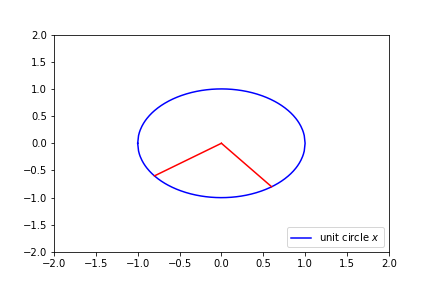
\includegraphics[scale=.6]{53circ.png}
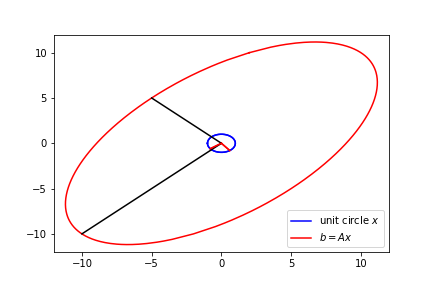
\includegraphics[scale=.6]{53elip.png}
\end{center}
\item We now consider,
\begin{enumerate}
\item $||A||_2=\sigma_1=10\sqrt{2}$
\item $||A||_F=\sqrt{200+50}=5\sqrt{10}$
\item $||A||_1=16$
\item $||A||_{\infty}=15$
\end{enumerate}
\item Now, we consider noting that $U$ and $V$ are unitary,
\[A^{-1}=(U\Sigma V)^{-1}=V^T \Sigma^{-1} U^T=\begin{bmatrix}
1/20 & -11/100\\ 1/10 & -1/50
\end{bmatrix}\]
\item We now compute the eigenvalues of $A$ as,
\begin{align*}
0=\begin{vmatrix}
-2-\lambda & 11\\
-10 & 5-\lambda
\end{vmatrix}&=(-2-\lambda)(5-\lambda)+110\\
&=\lambda^2-3\lambda+100\\
\lambda &= \frac{3\pm \sqrt{391}i}{2}
\end{align*}
\item Next, we compute,
\[det(A)=-2(5)+110=100\]
\[\lambda_1\lambda_2=\frac{3+\sqrt{391}i}{2}\frac{3-\sqrt{391}i}{2}=\frac{9+391}{4}=100\]
Thus, we see that $det(A)=\prod_i \lambda_i$ as desired.\\
We also consider, 
\[\sigma_1\sigma_2=(10\sqrt{2})(5\sqrt{2})=50(2)=100=|det(A)|\]
As desired.
\item Finally, we note that the area of the ellipsoid that $A$ maps our unit ball onto is $A=\pi \prod_i||v_i||$. We note that $||v_i||=\sigma_i$. Thus, our area formula becomes,
\[A=\pi\prod_i\sigma_i\]
For our ellipse, we compute,
\[A=\pi(100)\approx 314.1592653\] 
\end{enumerate}
\end{enumerate}
\end{document}
